\documentclass[convert={imagemagick, density=1024}]{standalone}
\usepackage{amsmath, amsthm, amsfonts,mathrsfs}
\usepackage{tikz-cd, kotex,tikz-3dplot}
\usepackage{../../.preamble/quiver}
\usepackage{../../.preamble/Operators}
\usetikzlibrary{arrows.meta}
\begin{document}

%% Spectrum/Peterson 동형: flag y = character = evaluation (Richardson_Peterson_Variety-1.png)
\begin{tikzcd}[row sep=2.8em, column sep=3.6em]
\mathbb{C}[q] \arrow[r, hook] \arrow[d, "\operatorname{ev}_{q_0}"'] & QH^\ast(G/P) \arrow[r, "\Phi", "\sim"'] \arrow[d, "\chi_y" description] & \mathbb{C}[\mathcal{Y}^\vee_P] \arrow[d, "\operatorname{ev}_y"] \\
\mathbb{C} \arrow[r, equal] & \mathbb{C} \arrow[r, equal] & \mathbb{C}
\end{tikzcd}

\end{document}

%% ===== 이전 다이어그램 보관 (archive; \end{document} 이후라 컴파일되지 않음) =====
%% Hasse diagram of Bruhat order for Gr(2,4) (Bruhat_Decomposition-1.png)
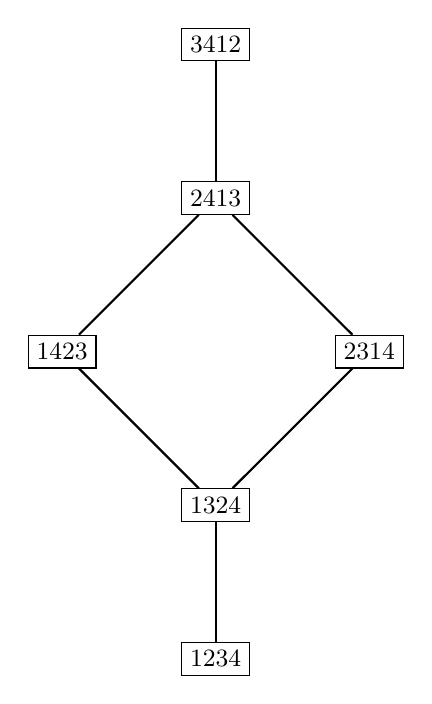
\begin{tikzpicture}[
    scale=1.3,
    node/.style={draw, fill=white, inner sep=3pt, font=\small},
    edge/.style={thick}
]
    % Nodes
    \node[node] (n0) at (0,0) {$1234$};
    \node[node] (n1) at (0,1.5) {$1324$};
    \node[node] (n2a) at (-1.5,3) {$1423$};
    \node[node] (n2b) at (1.5,3) {$2314$};
    \node[node] (n3) at (0,4.5) {$2413$};
    \node[node] (n4) at (0,6) {$3412$};

    % Edges
    \draw[edge] (n0) -- (n1);
    \draw[edge] (n1) -- (n2a);
    \draw[edge] (n1) -- (n2b);
    \draw[edge] (n2a) -- (n3);
    \draw[edge] (n2b) -- (n3);
    \draw[edge] (n3) -- (n4);
\end{tikzpicture}
